\documentclass[a4paper,12pt]{article} % добавить leqno в [] для нумерации слева
\usepackage[a4paper,top=1.3cm,bottom=2cm,left=1.5cm,right=1.5cm,marginparwidth=0.75cm]{geometry}
%%% Работа с русским языком
\usepackage{cmap}					% поиск в PDF
\usepackage[warn]{mathtext} 		% русские буквы в фомулах
\usepackage[T2A]{fontenc}			% кодировка
\usepackage[utf8]{inputenc}			% кодировка исходного текста
\usepackage[english,russian]{babel}	% локализация и переносы
\usepackage{multirow}
\usepackage{float}
\restylefloat{table}


%\graphicspath{ {images/}}
\usepackage{graphicx}

\usepackage{wrapfig}
\usepackage{tabularx}

\usepackage{hyperref}
\usepackage[rgb]{xcolor}
\hypersetup{
	colorlinks=true,urlcolor=blue
}

%%% Дополнительная работа с математикой
\usepackage{amsmath,amsfonts,amssymb,amsthm,mathtools} % AMS
\usepackage{icomma} % "Умная" запятая: $0,2$ --- число, $0, 2$ --- перечисление

%% Номера формул
\mathtoolsset{showonlyrefs=true} % Показывать номера только у тех формул, на которые есть \eqref{} в тексте.

%% Шрифты
\usepackage{euscript}	 % Шрифт Евклид
\usepackage{mathrsfs} % Красивый матшрифт

%% Свои команды
\DeclareMathOperator{\sgn}{\mathop{sgn}}

%% Перенос знаков в формулах (по Львовскому)
\newcommand*{\hm}[1]{#1\nobreak\discretionary{}
	{\hbox{$\mathsurround=0pt #1$}}{}}

\date{\today}

\title{Лабораторная работа 1.3.1. Определение модуля Юнга на основе
исследования деформаций растяжения и изгиба}
\date{}
\begin{document}
\maketitle
\section{Аннотация}
\subsection{Цели работы}
Экспериментально получить зависимость между напряжением и деформацией (закон Гука) для двух простейших напряженных состояний упругих тел: одноосного растяжения и чистого изгиба; по результатам измерений вычислить модуль Юнга.
\subsection{Ожидаемые результаты}
Получим зависимости между напряжением и деформацией, с помощью измерений и построенных графиков определим модуль Юнга для различных тел. Сравнивая полученное экспериментально значение модуля Юнга для проволоки с табличными значениями, определим материал, из которого она изготовлена.
\section{Теоретические сведения}
\textbf{Общие сведения:}
Внутренними напряжениями называются силы, возникающие при деформировании тела и стремящиеся вернуть его в первоначальное положение, отнесенные к соответстующим площадям.
Деформация -- это относительное смещение двух точек, деленное на первоначальное расстояние между ними, в точке по определению: \[\varepsilon = \frac{ds}{dx}\]

Напряжение, соответсвующее виду силы (растяжение (сжатие) либо сдвиг) определяется как сила, отнесенная к единице соответствующей площади: \[\sigma = \frac{F}{S}\]\\
Понятие напряжения имеет перед понятием силы то преимущество, что его можно установить в каждой точке (локальный вектор силы, дейстующий на единицу площади).\\
В общем случае, напряжение -- тензор второго ранга.

\textbf{Модули угругости:}
\(\varepsilon\) и \(\sigma\) связывают следующие, эмпирически выведенные соотношения:
для растяжения (сжатия): \(\sigma = E\varepsilon\), для сдвига: \(\sigma = G\varepsilon = G\gamma\)   (\(\gamma\) -- угол сдвига).\
E -- модуль Юнга, G -- модуль сдвига. Эти величины характеризуют упругие свойства материала твердого тела в области линейной зависимости напряжения и деформации. В нашем случае модуль Юнга для проволоки будет вычисляться следующим образом: \[E = \frac{lk}{S}\]
\subsection{Определение модуля Юнга по измерениям растяжения проволоки}

Эта часть работы описывается формулой, так как производят расстяжение проволки, что соответствует случаю одноосного напряженного состояния:
\[
    \sigma = E \cdot \varepsilon~\text{ , где } \sigma = \frac{F}{S}
\]
Для определения модуля Юнга используется прибор Лермантова:

\begin{figure}[H]
    \centering
    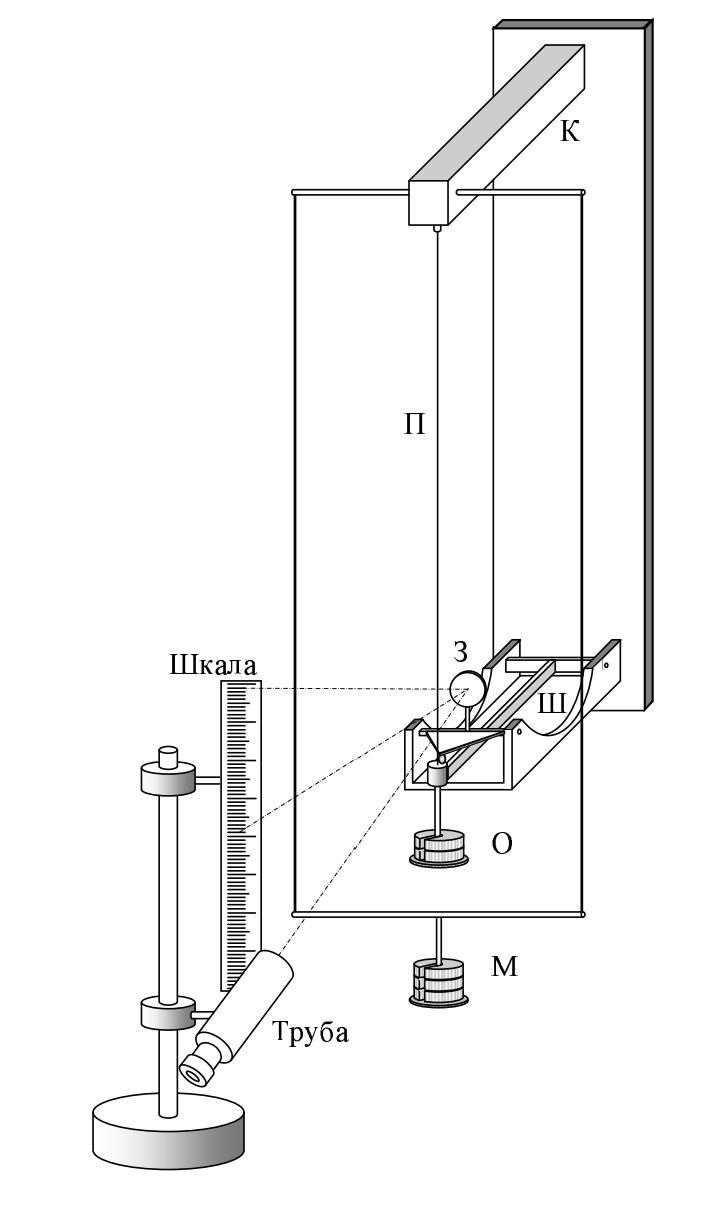
\includegraphics[width=0.4\textwidth]{images/1.png}
\end{figure}

Верхний конец проволоки \text{П}, изготовленной из исследуемого материала, прикреплен к консоли \textbf{К}, а нижний - к цилиндру, которым оканчивается шарнирный кронштейн \textbf{Ш}. На этот же цилиндр опирается рычаг \text{r}, связанный с зеркальцем \textbf{3}. Таким образом, удлинение проволоки можно измерить по углу поворота зеркальца.

Натяжение проволоки можно менять, перекладывая грузы с площадки М на площадку О и наоборот. Такая система позволяет исключить влияние деформации кронштейна К на точность измерений, так как нагрузка на нем все время остается постоянной.
При проведении эксперимента следует иметь в виду, что проволока П при отсутствии нагрузки всегда несколько изогнута, что не может не сказаться на результатах, особенно при небольших нагрузках. Проволока вначале не столько растягивается, сколько распрямляется.\\
Формулу, связывающую число делений по шкале $n$, расстояние $h$ от шкалы до зеркальца, длину рычага $r$ и удлинение можно выразить ис следующих соображений:\\
Если направить зрительную трубу на зеркальце так, чтобы мы четко видели шкалу, тогда свет от шкалы будет падать примерно перпендикулярно шкале на зеркало, поэтому
\[
    \Delta l =\dfrac{nr}{2h}
\]
Модуль Юнга можем посчитать по формуле, где $k$ угол наклона прямой зависимости удлинения от прикладываемой силы:
\[
    E = \frac{kl_0}{S}
\]
\begin{equation}
    \sigma_E = \sqrt{\left( \dfrac{\sigma_{k}}{k} \right)^2 + \left( \dfrac{\sigma_{S}}{S} \right)^2 + \left( \dfrac{\sigma_{l_0}}{l_0} \right)^2 }
\end{equation}

\subsection{Определение модуля Юнга по измерениям изгиба балки}

Экспериментальная установка состоит из стойки с опорными призмами А и Б:

\begin{figure}[H]
    \centering
    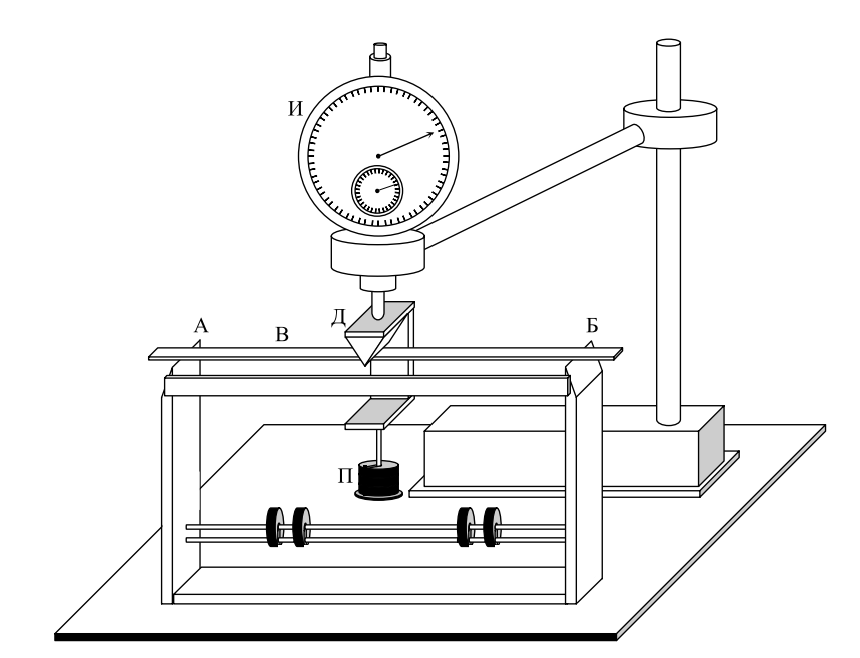
\includegraphics[height=0.4\textheight]{images/2.png}
\end{figure}

На ребра призм опирается исследуемый стержень (балка) В. В середине стержня на призме Д подвешена площадка П с грузами. 

Измерять стрелу прогиба можно с помощью индикатора И, укрепляемого на отдельной штанге. Полный оборот большой стрелки индикатора соответствует 1 мм и одному делению малого циферблата.

Модуль Юнга Е материала стержня связан со стрелой прогиба $Y_{max}$ (то есть с перемещением середины стержня) следующим соотношением:

\begin{equation} \label{1}
    E = \frac {Pl^3}{4ab^3y_{max}}
\end{equation}

Здесь $ P $  - нагрузка, вызывающая прогиб стержня, $ l $  - расстояние между призмами А и Б, а и - ширина и высота сечения стержня.

Формула \eqref{1} была выведена при условиях, что, во-первых, ребра опорных призм А и Б находятся на одной горизонтали (высоте) и, во-вторых, сила $ P $  приложена точно посередине балки.

\section{Методика измерений}
\begin{enumerate}
    \item \begin{enumerate}
        \item Измеряем площадь поперечного сечения проволоки с помощью микрометра
        \item Измеряем длину проволоки 
        \item Измеряем расстояние от шкалы до зеркальца
        \item Оцениваем максимальную величину нагрузки
        \item Измеряем зависимость $ n(m) $ 2 раза
        \item Строим график $\delta l (P)$
        \item  Из графика получаем модуль Юнга
        \item Сравниваем с табличным
    \end{enumerate}
    \item \begin{enumerate}
        \item Измеряем расстояние AB
        \item Снимаем зависимость $ y_{\max}(P)$, переворачиваем и снимаем снова. Повторяем это для стержней различных материалов
        \item Для каждого стержня строим график и извлекаем модуль Юнга
        \item Сравниваем с табличным
    \end{enumerate}
\end{enumerate}

\section{Используемое оборудование}
\textbf{В работе используется следующее оборудование:} в первой части -- прибор Лермантова, проволока из исследуемого материала, зрительная труба со шкалой,
набор грузов, микрометр, рулетка; во второй части -- стойка для
изгибания балки, индикатор для измерения величины прогиба, набор
исследуемых стержней, грузы, линейка, штангенциркуль.

\textbf{Погрешности измерений:}  \begin{enumerate}
    \item штангенциркуль 0.05 мм
    \item микрометр 0.01 мм
    \item двухметровая линейка/рулетка 0.1 см
    \item прибор Лермантова $ 2\% $ (относительная погрешность)
    \item установка для измерения прогиба балки 0.01 мм 
\end{enumerate}
\section{Результаты измерений}
\begin{table}[!ht]
    \centering
    \begin{tabular}{|c|c|c|c|c|c|c|c|c|c|c}
        \hline
    $ P $   & ~~~ & ~~~ & ~~~ & ~~~ & ~~~ & ~~~ & ~~~ &  ~~~ \\ \hline
    $y_{max}$ & ~~~ & ~~~ & ~~~ & ~~~ & ~~~ & ~~~ & ~~~ &  ~~~\\ \hline
    \end{tabular}
    \caption{Стержень 1 центральное}
\end{table}
\begin{table}[!ht]
    \centering
    \begin{tabular}{|c|c|c|c|c|c|c|c|c|c|c}
        \hline
    $ P $   & ~~~ & ~~~ & ~~~ & ~~~ & ~~~ & ~~~ & ~~~ &  ~~~ \\ \hline
    $y_{max}$ & ~~~ & ~~~ & ~~~ & ~~~ & ~~~ & ~~~ & ~~~ &  ~~~\\ \hline
    \end{tabular}
    \caption{Стержень 1 сдвинутое}
\end{table}
\begin{table}[!ht]
    \centering
    \begin{tabular}{|c|c|c|c|c|c|c|c|c|c|c}
        \hline
    $ P $   & ~~~ & ~~~ & ~~~ & ~~~ & ~~~ & ~~~ & ~~~ &  ~~~ \\ \hline
    $y_{max}$ & ~~~ & ~~~ & ~~~ & ~~~ & ~~~ & ~~~ & ~~~ &  ~~~\\ \hline
    \end{tabular}
    \caption{Стержень 2 центральное}
\end{table}
\begin{table}[!ht]
    \centering
    \begin{tabular}{|c|c|c|c|c|c|c|c|c|c|c}
        \hline
    $ P $   & ~~~ & ~~~ & ~~~ & ~~~ & ~~~ & ~~~ & ~~~ &  ~~~ \\ \hline
    $y_{max}$ & ~~~ & ~~~ & ~~~ & ~~~ & ~~~ & ~~~ & ~~~ &  ~~~\\ \hline
    \end{tabular}
    \caption{Стержень 2 сдвинутое}
\end{table}
\begin{table}[!ht]
    \centering
    \begin{tabular}{|c|c|c|c|c|c|c|c|c|c|c}
        \hline
    $ P $   & ~~~ & ~~~ & ~~~ & ~~~ & ~~~ & ~~~ & ~~~ &  ~~~ \\ \hline
    $y_{max}$ & ~~~ & ~~~ & ~~~ & ~~~ & ~~~ & ~~~ & ~~~ &  ~~~\\ \hline
    \end{tabular}
    \caption{Стержень 3 центральное}
\end{table}
\begin{table}[!ht]
    \centering
    \begin{tabular}{|c|c|c|c|c|c|c|c|c|c|c}
        \hline
    $ P $   & ~~~ & ~~~ & ~~~ & ~~~ & ~~~ & ~~~ & ~~~ &  ~~~ \\ \hline
    $y_{max}$ & ~~~ & ~~~ & ~~~ & ~~~ & ~~~ & ~~~ & ~~~ &  ~~~\\ \hline
    \end{tabular}
    \caption{Стержень 3 сдвинутое}
\end{table}
\begin{table}[!ht]
    \centering
    \begin{tabular}{|c|c|c|c|c|c|c|c|c|c|c}
        \hline
    $ m $   & ~~~ & ~~~ & ~~~ & ~~~ & ~~~ & ~~~ & ~~~ &  ~~~ \\ \hline
    $n$ & ~~~ & ~~~ & ~~~ & ~~~ & ~~~ & ~~~ & ~~~ &  ~~~\\ \hline
    \end{tabular}
    \caption{Эксперимент 1}
\end{table}
\begin{table}[!ht]
    \centering
    \begin{tabular}{|c|c|c|c|c|c|c|c|c|c|c}
        \hline
    $ m $   & ~~~ & ~~~ & ~~~ & ~~~ & ~~~ & ~~~ & ~~~ &  ~~~ \\ \hline
    $ n $ & ~~~ & ~~~ & ~~~ & ~~~ & ~~~ & ~~~ & ~~~ &  ~~~\\ \hline
    \end{tabular}
    \caption{Эксперимент 2}
\end{table}

\end{document}